\section{Espacio de trabajo}

Para poder entender a donde se va a insertar al usuario, detallamos en esta pequeña sección el espacio en donde va a trabajar el usuario para mejorar. Mas específicamente se tratará de 2 porciones de una casa, la cocina y el living/comedor. En la Figura \ref{low_poly_house_interior} se puede observar el modelo del cual se partió para empezar a cambiar y agregarle nuevos componentes para que el usuario se sienta cómodo.

\begin{figure}[ht!]
    \centering
    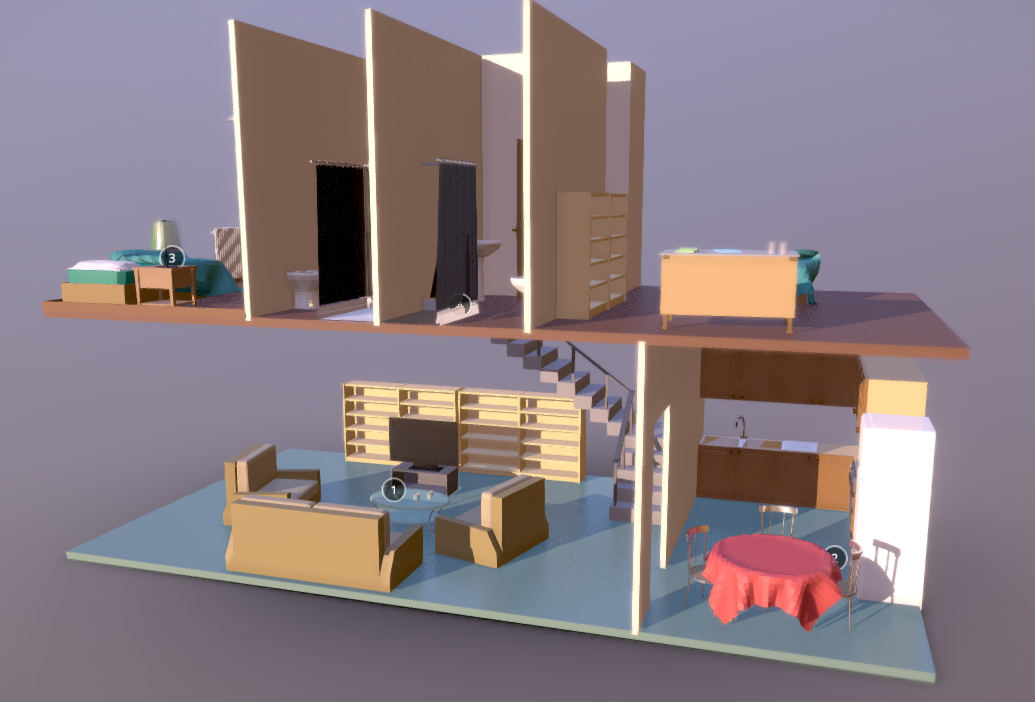
\includegraphics[width=0.7\textwidth]{figs/lowpoly_house_interior.png}
    \caption{Interior de Casa LowPoly}
    \label{low_poly_house_interior}
\end{figure}

Sin embargo, por las cuestiones mencionadas, solo se procedió a utilizar la planta baja, y el primer piso se lo descartó.

En la figura \ref{house_distribution} se observa lo que posteriormente fue la distribución de objetos en la planta baja entre los cuales el usuario tiene la posibilidad de cambiar, esto es para darnos una mejor idea de como es el espacio en donde nos vamos a encontrar ni bien ingresemos al mundo.

\begin{figure}[ht!]
    \centering
    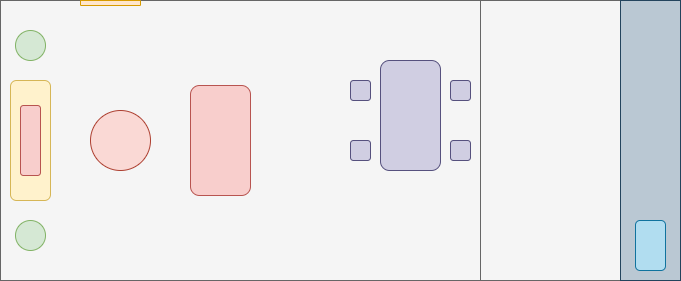
\includegraphics[width=0.7\textwidth]{figs/distribucion.png}
    \caption{Distribución de objetos}
    \label{house_distribution}
\end{figure}

Como se pueden ver en la imagen hay diferentes tipos de cosas que se pueden cambiar a continuación se enumeraran algunas de ellas:

\begin{itemize}
    \item Rojo: Sillones
    \item Rojo: Mesa Ratona
    \item Rojo: Televisión
    \item Amarillo: Mueble televisión
    \item Verdes: Muebles decoraciones
    \item Amarillo: Pintura en la pared
    \item Violeta: Mesa comedor
    \item Violeta: Sillas comedor
    \item Celeste: Microondas
\end{itemize}

Sin embargo, hay cosas que no se pueden ver en el plano de la figura \ref{house_distrib} debido a que no se ven desde esa vista, esas cosas son por ejemplo las lamparas de techo y las decoraciones sobre los muebles. Por otro lado, otra pata importante sobre el diseño es tener la posibilidad de cambiar los materiales, y es por esto que también tenemos la posibilidad de cambiarle los materiales a:

\begin{itemize}
    \item Todas las paredes independientes entre sí
    \item Ambos techos (living y cocina)
    \item Ambos suelos (living y cocina)
    \item Marmol de la cocina
    \item Material muebles de cocina
\end{itemize}

A continuación en las figuras \ref{diseno_1}, \ref{diseno_2} y \ref{diseno_3} mostraremos algunos de los ejemplos de los diseños posibles de realizar con diferentes combinaciones de objetos y materiales.

\begin{figure}
     \centering
     \begin{subfigure}[b]{0.5\textwidth}
         \centering
         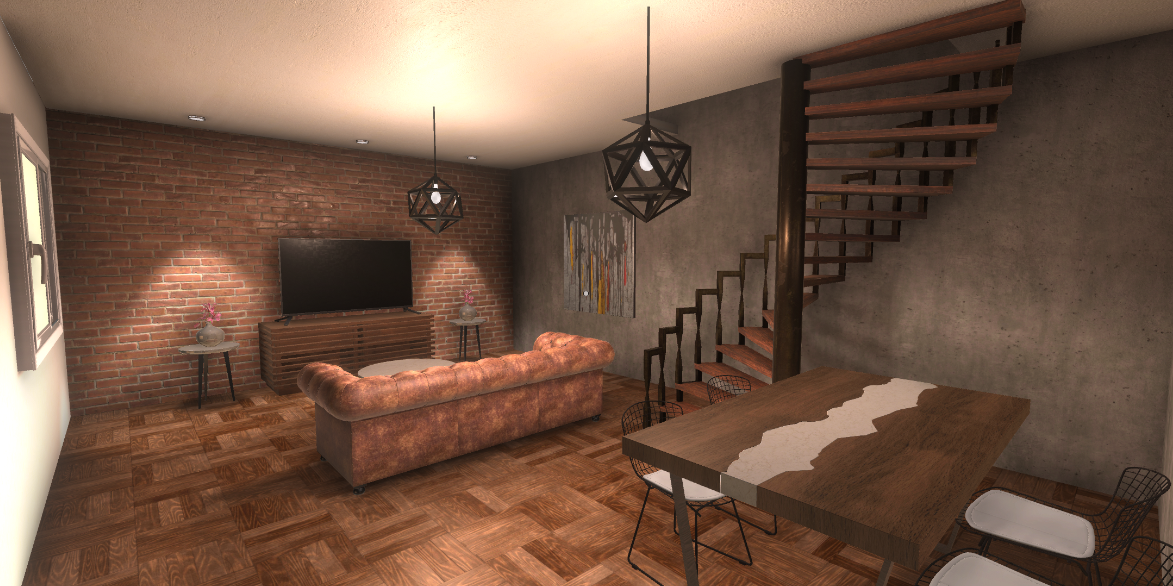
\includegraphics[width=\textwidth]{figs/1_1.png}
         \caption{Living}
         \label{1_1}
     \end{subfigure}
     \hfill
     \begin{subfigure}[b]{0.5\textwidth}
         \centering
         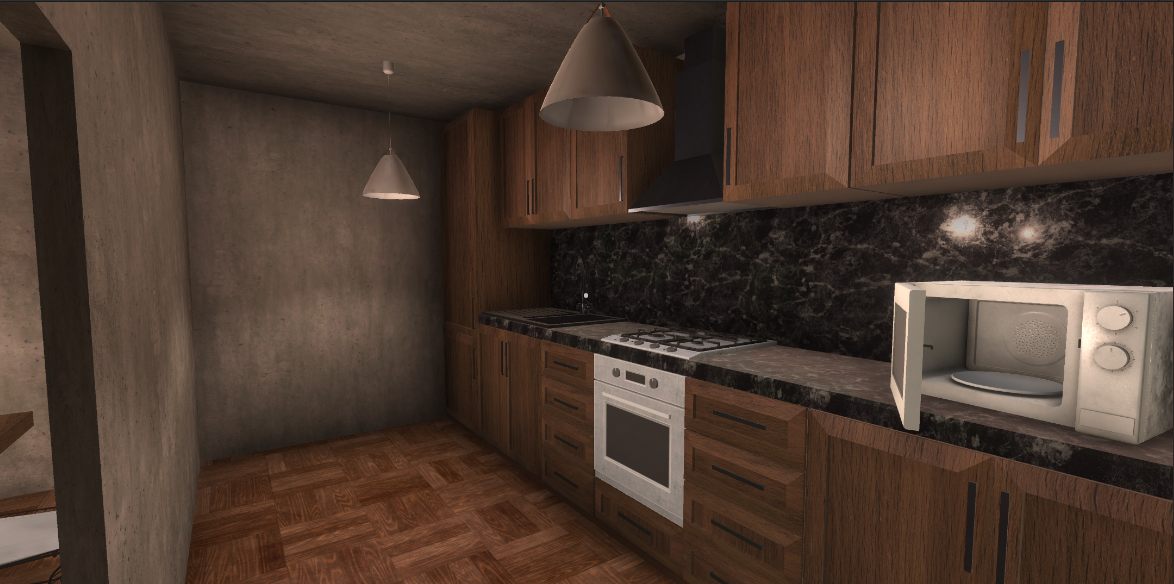
\includegraphics[width=\textwidth]{figs/1_2.png}
         \caption{Cocina}
         \label{1_2}
     \end{subfigure}
     \hfill
        \caption{Diseño Ejemplo 1}
        \label{diseno_1}
\end{figure}

\begin{figure}
     \centering
     \begin{subfigure}[b]{0.5\textwidth}
         \centering
         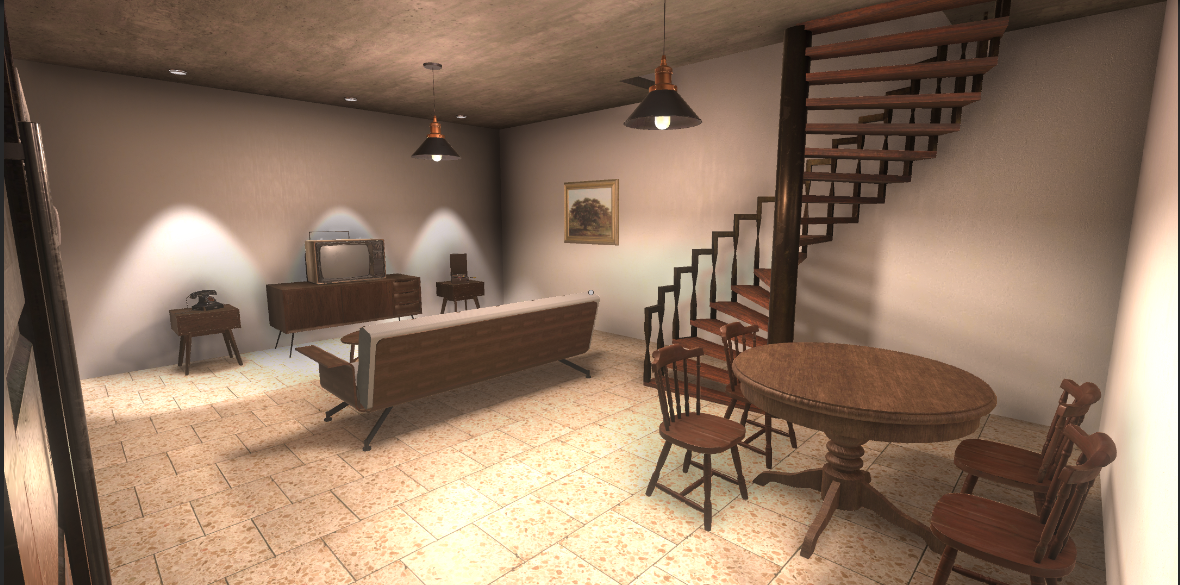
\includegraphics[width=\textwidth]{figs/2_1.png}
         \caption{Living}
         \label{1_1}
     \end{subfigure}
     \hfill
     \begin{subfigure}[b]{0.5\textwidth}
         \centering
         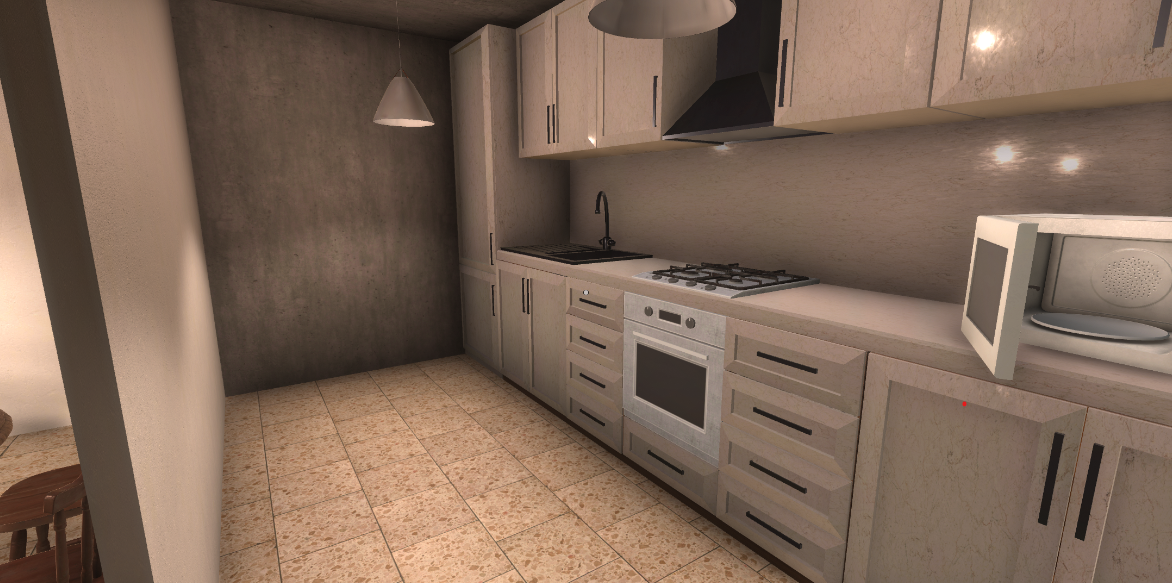
\includegraphics[width=\textwidth]{figs/2_2.png}
         \caption{Cocina}
         \label{1_2}
     \end{subfigure}
     \hfill
        \caption{Diseño Ejemplo 2}
        \label{diseno_2}
\end{figure}

\begin{figure}
     \centering
     \begin{subfigure}[b]{0.5\textwidth}
         \centering
         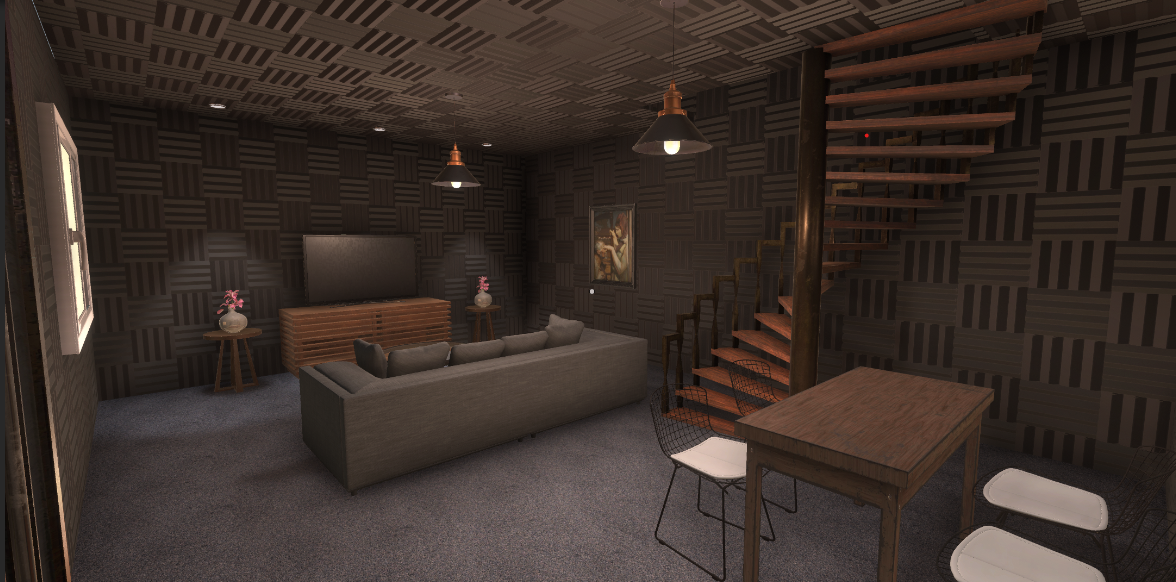
\includegraphics[width=\textwidth]{figs/3_1.png}
         \caption{Living}
         \label{1_1}
     \end{subfigure}
     \hfill
     \begin{subfigure}[b]{0.5\textwidth}
         \centering
         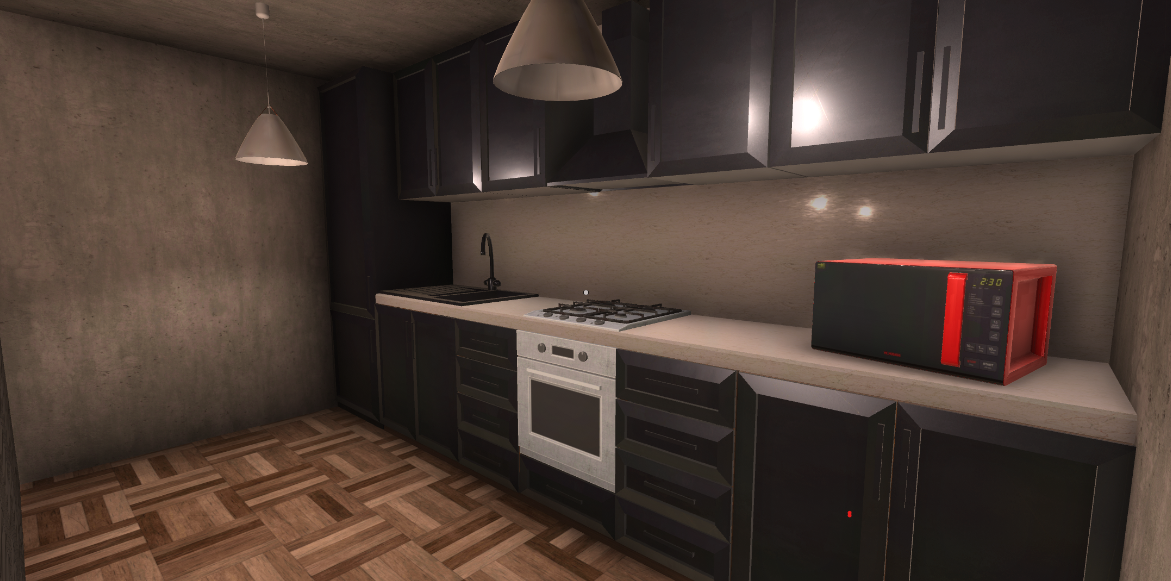
\includegraphics[width=\textwidth]{figs/3_2.png}
         \caption{Cocina}
         \label{1_2}
     \end{subfigure}
     \hfill
        \caption{Diseño Ejemplo 3}
        \label{diseno_3}
\end{figure}

